% !TEX TS-program = pdflatex
% !TEX encoding = UTF-8 Unicode
%
% Monotonic Math: A Provably Floor-Preserving Tokenomic Primitive
% for Revenue-Bearing On-Chain Assets.
% (Reduced 15-page variant; see README.md for the source it was reduced from.)

\documentclass[11pt,a4paper]{article}

\usepackage[utf8]{inputenc}
\usepackage[T1]{fontenc}
\usepackage{lmodern}
\usepackage{microtype}
\linespread{0.97}
\usepackage[a4paper,margin=0.85in]{geometry}
\usepackage{amsmath,amssymb,amsthm}
\usepackage{mathtools}
\usepackage{stmaryrd}  % provides \llbracket, \rrbracket used by \contractEval
\usepackage{booktabs}
\usepackage{array}
\setlength{\emergencystretch}{6em}
\usepackage{graphicx}
\graphicspath{{figures/}}
\usepackage{tikz}
\usetikzlibrary{positioning,arrows.meta,calc}
\usepackage{hyperref}
\usepackage{xcolor}
\usepackage{enumitem}
\setlist{nosep}
\usepackage{natbib}
\setlength{\bibsep}{1pt plus 0.2ex}
\usepackage{authblk}
\usepackage{caption}
\usepackage{titlesec}
\titlespacing*{\section}{0pt}{*1.4}{*0.6}
\titlespacing*{\subsection}{0pt}{*1.1}{*0.4}
\titlespacing*{\paragraph}{0pt}{*0.6}{1ex}

\hypersetup{
  colorlinks=true,
  linkcolor=blue!50!black,
  citecolor=blue!50!black,
  urlcolor=blue!50!black,
  pdftitle={Monotonic Math: A Provably Floor-Preserving Tokenomic Primitive for Revenue-Bearing On-Chain Assets},
  pdfauthor={Mostafa Sadjadi},
  pdfsubject={Tokenomics; decentralized finance; mechanism design; automated market makers},
  pdfkeywords={tokenomics, DeFi, AMM, redemption mechanics, closed-end funds, capital returns},
}

% ----- Theorem environments -----
\theoremstyle{plain}
\newtheorem{theorem}{Theorem}
\newtheorem{lemma}[theorem]{Lemma}
\newtheorem{corollary}[theorem]{Corollary}
\newtheorem{proposition}[theorem]{Proposition}
\newtheorem{conjecture}[theorem]{Conjecture}

\theoremstyle{definition}
\newtheorem{definition}[theorem]{Definition}
\newtheorem{assumption}[theorem]{Assumption}

\theoremstyle{remark}
\newtheorem{remark}[theorem]{Remark}

% ----- Notation macros (preserved verbatim from source) -----
\newcommand{\Tres}{T}              % Treasury stable
\newcommand{\Sup}{S}               % Total supply
\newcommand{\Lt}{L_t}              % LP token reserves
\newcommand{\Ls}{L_s}              % LP stable reserves
\newcommand{\Floor}{F}             % Floor price T/S
\newcommand{\Spot}{P}              % Spot price L_s/L_t
\newcommand{\kInv}{k}              % Constant-product invariant
\newcommand{\Phit}{\Phi_t}         % Unrealized token-side fee accumulator
\newcommand{\Phis}{\Phi_s}         % Unrealized stable-side fee accumulator
\newcommand{\Kreal}{K}             % Realized token-side fees (gross)
\newcommand{\Ureal}{U}             % Realized stable-side fees (gross)
\newcommand{\Qprec}{Q}             % 10^18 precision factor
\newcommand{\dstab}{d_s}           % Stable's decimals
\newcommand{\Qstab}{Q_s}           % 10^{d_s}
\newcommand{\contractEval}[1]{\llbracket #1 \rrbracket}  % Integer-faithful evaluation

% ----- Title block -----
\title{Monotonic Math: A Provably Floor-Preserving Tokenomic Primitive for Revenue-Bearing On-Chain Assets}

\author{Mostafa Sadjadi\thanks{Correspondence: \texttt{0xmostafas@proton.me}. ORCID: \href{https://orcid.org/0009-0005-2573-3336}{0009-0005-2573-3336}. Funding and conflict-of-interest statements appear in the \emph{Disclosures} section preceding the bibliography.}}
\affil{Independent Researcher}

\date{May 27, 2026}

\begin{document}
\maketitle

\begin{abstract}
We present \emph{Monotonic Math} (M\textsuperscript{2}), a tokenomic primitive combining a fixed-supply redemption-backed token, an asymmetric-fee AMM, and a hardcoded revenue router to enforce a contractually monotone non-decreasing redemption floor (conditional on contract correctness and stablecoin solvency). Under every protocol-defined operation, the per-token reserve claim is provably non-decreasing. We prove this by case analysis and derive a closed-form saturation quantity above which the optimal dump-portion of any \emph{simultaneous} composite attacker strategy is bounded by a state-only constant independent of holdings---a Diamond--Dybvig analogue with reversed conclusion: later redeemers weakly dominate earlier ones. We characterize the operating envelope through closed-form deterministic projections and stochastic-revenue bands over the four free parameters, with a Hardhat v3 invariant-test cross-track in CI. The mechanism composes three TradFi instruments that, to our knowledge, do not coexist in any single offering: a NAV-redemption closed-end fund, a sponsor-funded perpetual buyback, and a Pigovian sell tax recycled into common-pool value.
\end{abstract}

\noindent\textbf{Keywords:} tokenomics, decentralized finance, mechanism design, automated market makers, redemption mechanics, capital returns, closed-end funds.

\medskip\noindent\textbf{Reproducibility.} Simulator code and figure-generation scripts: Zenodo DOI \href{https://doi.org/10.5281/zenodo.20255141}{\texttt{10.5281/zenodo.20255141}}. Git tag \texttt{v0.2.0-paper-v2} pins the version cited.

% ============================================================
% ============================================================
\section{Introduction}
\label{sec:introduction}

Public equities have a disciplined vocabulary for returning capital---dividends, buybacks, redeemable instruments---backed by securities law and fiduciary duty. Tokens on programmable blockchains inherit none of that enforcement: the language of TradFi capital returns has repeatedly been used on-chain without the primitives that made those returns credible \citep{LiuMakarovSchoar2023,KlagesMundtMinca2021}. This paper exhibits the simplest on-chain primitive that closes the gap and proves the gap is closed.

We present \emph{Monotonic Math} (M\textsuperscript{2}), a tokenomic primitive composed of four immutable contracts: a fixed-supply ERC-20 with \texttt{redeem}, a passive stablecoin treasury with no admin withdraw, an asymmetric-fee AMM as a Uniswap v4 hook \citep{UniswapV4}, and a revenue router with a hardcoded $50/50$ split. The load-bearing property is \emph{floor monotonicity}: under every protocol-defined operation, the per-token claim $\Floor = \Tres/\Sup$ is non-decreasing (Theorem~\ref{thm:floor-monotonicity}). The property is structural: it depends only on contract code and stablecoin solvency, not on holder coordination or operator discretion.

\textbf{C1 (Primitive).} A complete deployable protocol with four immutable contracts and four free parameters; the genesis constraint $\Tres_0/\Sup_0 = L_{s,0}/L_{t,0}$ pins $\Floor_0 = \Spot_0$. \textbf{C2 (Proofs).} Floor monotonicity (Theorem~\ref{thm:floor-monotonicity}); integer-arithmetic redemption (Lemma~\ref{lem:integer-redemption}); composite-strategy bank-run with state-only saturation (Theorem~\ref{thm:bank-run}); redemption fairness inverting the \citet{ChenGoldsteinJiang2010} first-mover advantage of Diamond--Dybvig \citep{DiamondDybvig1983} (Theorem~\ref{thm:redemption-fairness}); LP half-life (Theorem~\ref{thm:lp-half-life}); \texttt{collectFees} calling equilibrium (Theorem~\ref{thm:collect-equilibrium}); MEV leakage (Theorem~\ref{thm:mev-bound}); spot--floor convergence under revenue cessation (Theorem~\ref{thm:spot-floor-convergence}); a directional LVR inversion of \citet{MilionisMoallemiRoughgarden2023} (Conjecture~\ref{conj:lvr-capture}). \textbf{C3 (Quantitative envelope).} Two-track simulator in CI: NumPy/Decimal Track~A and Hardhat~v3 invariant-fuzz Track~B over compiled bytecode, agreement enforced at \texttt{ABS\_TOL = 1e-3}, \texttt{REL\_TOL = 1e-9}; divergence is paper-stopping.

\noindent\textbf{What we do not claim.} Spot-price monotonicity, immunity to backing-stable issuer failure, operator-fraud robustness, end-to-end mechanized verification, token-return predictions, and regulatory classification.

% ============================================================
\section{Background and Positioning}
\label{sec:related-work}

M\textsuperscript{2} sits at four literatures' intersection. \emph{TradFi capital returns}---buybacks \citep{GrullonMichaely2002}, retractable bonds \citep{BrennanSchwartz1977}, closed-end funds whose persistent discount-to-NAV \citep{LeeShleiferThaler1991,Pontiff1996,CherkesSagiStanton2009} reflects the absence of contract-level NAV-redemption---supply the design language. \emph{CFMM theory} \citep{Angeris2020,UniswapV4} supplies the AMM algebra; \emph{MEV} \citep{Daian2020} the anti-MEV mitigations of Section~\ref{sec:protocol}. \emph{Stablecoin runs}---Terra--Luna \citep{LiuMakarovSchoar2023}---supply the canonical negative analog.

\paragraph{Four structural inversions.} (i) The \citet{ChenGoldsteinJiang2010} first-mover advantage driving Diamond--Dybvig \citep{DiamondDybvig1983} dynamics is absent: Theorem~\ref{thm:redemption-fairness} shows later redeemers weakly dominate. (ii) Terra--Luna's endogenous-collateral feedback \citep{LiuMakarovSchoar2023,Briola2023} is structurally absent: M\textsuperscript{2}'s backing is exogenous and inflow is one-way (Theorem~\ref{thm:bank-run}). (iii) The persistent CEF discount-to-NAV \citep{LeeShleiferThaler1991,Pontiff1996,CherkesSagiStanton2009} is bounded above under zero revenue, net-sell pressure, and a positive-probability arbitrageur path: Theorem~\ref{thm:spot-floor-convergence}(3) bounds $D(t)$'s limit above by $f_b \cdot \Floor$. (iv) LVR \citep{MilionisMoallemiRoughgarden2023} flips sign for a protocol-owned LP: the asymmetric fee folds LVR-equivalent value into the floor (Conjecture~\ref{conj:lvr-capture}; quantitative completion is P2).

% ============================================================
\section{Protocol Specification}
\label{sec:protocol}

This section specifies M\textsuperscript{2} as a deployable system: four immutable contracts, a genesis ceremony, the operations they expose, and a threat model that delimits the conditions under which the formal guarantees of Section~\ref{sec:formal-invariants} hold. Notation follows Appendix~\ref{app:symbols}.

\paragraph{System.} M\textsuperscript{2} is composed of four contracts---a token, a treasury, an asymmetric-fee LP hook, and a revenue router---together with one off-protocol \emph{operator} who routes business revenue (denominated in the backing stable) into the router.\footnote{The Solidity reference implementation is at the Zenodo artifact referenced in the abstract; the bytecode is the contract.} Each contract is deployed once with no admin key, governance hook, upgrade path, or parameter-change interface. Figure~\ref{fig:architecture} shows the system. Dynamics: (i) the operator deposits revenue $X$ into the router, which atomically deposits $X/2$ into the treasury and uses $X/2$ for a buy-and-burn on the protocol-owned LP; (ii) holders invoke either \texttt{redeem} on the token (atomic, no cooldown, no fee) or an LP swap (asymmetric per-direction fee enforced by the hook); (iii) any external caller may invoke \texttt{collectFees}, which routes $99.75\%$ of token-side fees to burn and $99.75\%$ of stable-side fees to the treasury, with $0.25\%$ per side paid as a caller bounty.

\begin{figure}[t]
\centering
\resizebox{0.6\textwidth}{!}{%
\begin{tikzpicture}[
  node distance=1.5cm and 2.0cm,
  contract/.style={draw, thick, rounded corners=2pt, minimum width=3.2cm, minimum height=0.9cm, align=center, font=\small},
  business/.style={draw, thick, dashed, rounded corners=2pt, minimum width=2.4cm, minimum height=0.6cm, align=center, font=\small},
  every node/.style={font=\small},
  flow/.style={->, thick, >=stealth},
  feeflow/.style={->, thick, >=stealth, dashed, gray!70!black},
  immut/.style={fill=blue!5},
]
  \node[contract, immut] (token) {Token (ERC-20) \\ \scriptsize fixed supply $\Sup_0=10^9$, burn, redeem};
  \node[contract, immut, right=of token] (treas) {Treasury \\ \scriptsize stable reserve $\Tres$, one-way in};
  \node[contract, immut, below=of token] (hook) {LP + V4 Hook \\ \scriptsize asym.\ fees, anti-MEV};
  \node[contract, immut, below=of treas] (router) {Revenue Router \\ \scriptsize 50/50 split, immutable};
  \node[business, below=0.9cm of router] (biz) {Business};
  \draw[flow] (token) -- node[above, font=\scriptsize]{redeem} (treas);
  \draw[flow] (hook) -- node[left, font=\scriptsize]{burn} (token);
  \draw[flow] (router) -- node[above, font=\scriptsize]{50\%} (treas);
  \draw[flow] (router) -- node[above, font=\scriptsize]{50\%, buy} (hook);
  \draw[flow] (biz) -- node[right, font=\scriptsize]{routeRevenue} (router);
  \draw[feeflow] (hook.west) to[out=180, in=200, looseness=1.5]
      node[left, font=\scriptsize, align=right]{collectFees:\\token burn} (token.west);
  \draw[feeflow] (hook.south east) to[out=-20, in=-90, looseness=1.4]
      node[below right=2pt, font=\scriptsize, align=left]{collectFees:\\stable to $\Tres$} (treas.south east);
\end{tikzpicture}}
\caption{System architecture. Blue-tinted boxes are immutable contracts; the dashed box is the off-protocol operator. Solid arrows mark primary flows; dashed gray arrows mark the permissionless \texttt{collectFees} realization paths (token side: $99.75\%$ burned, $0.25\%$ to caller; stable side: $99.75\%$ to treasury, $0.25\%$ to caller). All inflows to Treasury are one-way: stablecoin can leave only via \texttt{redeem}, which simultaneously burns the redeemed tokens.}
\label{fig:architecture}
\end{figure}

\paragraph{Token, redemption, floor precision.} The token is an ERC-20 with $18$ decimals and total supply $\Sup_0 = 10^9$ minted to the deployer in a single transaction; the constructor-set genesis-mint sentinel blocks all further minting. Three callers can \texttt{burn}: the hook (token-side LP fees), the router (buy-and-burn), and the token's own \texttt{redeem}. \texttt{redeem(uint256 amount)} is atomic, non-pausable, with no cooldown, fee, or maximum: it burns the caller's tokens, computes the payout as $\texttt{amount} \times \texttt{floorPrice}()$, and instructs the treasury to transfer via the privileged \texttt{payRedemption} interface. The floor returns an 18-decimal fixed-point value regardless of the stable's native decimals $\dstab$:
\begin{equation}
\texttt{floorPrice}() = \frac{\Tres \cdot 10^{18 + 18 - \dstab}}{\Sup},
\label{eq:floor-precision}
\end{equation}
with the wide intermediate in \texttt{uint256}; $10^{42} \ll 2^{256}$ rules out overflow. Integer truncation can leave at most $\Sup - 1$ smallest units of dust in the treasury's favor per call; Lemma~\ref{lem:integer-redemption} shows the residual strictly raises the floor. The treasury exposes exactly one privileged entry point, \texttt{payRedemption}, callable only by the token contract; no admin, withdraw, pause, upgrade, or governance hook. Stablecoin leaves only through \texttt{payRedemption} in lockstep with a token burn.

\paragraph{Asymmetric-fee hook and V2-equivalent algebra.} The protocol-owned LP is a Uniswap v4 pool initialized with \texttt{DYNAMIC\_FEE\_FLAG} and a single \emph{full-range} position spanning $[\text{MIN\_TICK}, \text{MAX\_TICK}]$. Under this configuration v4's active liquidity equals the position's at every reachable price and per-tick concentrated-liquidity bookkeeping never engages: $(\Lt, \Ls)$ are V2-style reserves of a single piecewise-constant liquidity segment, and $\kInv = \Lt \cdot \Ls$ is exact modulo the asymmetric-fee deduction. The position-owning contract has no removal interface, so liquidity is provably unwithdrawable. On every swap, the hook's \texttt{beforeSwap} returns a fee override determined by direction:
\begin{equation}
\text{fee}(\text{direction}) =
\begin{cases}
0.10\% & \text{if input is stable (buy)} \\
3.00\% & \text{if input is token (sell)}
\end{cases}
\label{eq:fee-asymmetry}
\end{equation}
The fee is subtracted from input before the curve and folded into the input-side accumulator, denoted $(\Phit, \Phis)$ in Section~\ref{sec:formal-invariants}.\footnote{V4 stores the accumulator as Q128.128 \texttt{feeGrowthGlobalX128}; the raw-token framing here is dimensionally equivalent.} The $3.00\%$ sell fee converts every adversarial LP exit into common-pool value. A holder's two exit paths are both floor-non-decreasing: \texttt{redeem} preserves the floor exactly (Case~3), and the LP-sell path holds it flat at swap and strictly raises it at the next \texttt{collectFees} (Cases~5,~7). Protocol-initiated buys use private-orderflow routing, a uniform delay $\tau \sim U[0, 12\,\text{h}]$, and optional TWAP splitting; residual MEV leakage is bounded by Theorem~\ref{thm:mev-bound} (Appendix~\ref{app:auxiliary}).

\paragraph{Revenue router and \texttt{collectFees} distribution.} The router exposes a single function callable only by the immutably-set depositor: it pulls a stable amount, deposits $\lfloor \cdot/2 \rfloor$ into the treasury, and uses $\lceil \cdot/2 \rceil$ for a buy-and-burn via the hook in the same transaction. The split is a bytecode constant---no setter, upgrade path, or governance hook. The hook exposes a permissionless \texttt{collectFees}: it acquires the pool-manager lock, calls \texttt{modifyLiquidity} with zero delta, obtains $(\Kreal, \Ureal) = (\Phit, \Phis)$, and distributes:
\begin{align}
\text{caller bounty (token):} \quad & K_b = \lfloor 0.0025 \cdot \Kreal \rfloor, \\
\text{caller bounty (stable):} \quad & U_b = \lfloor 0.0025 \cdot \Ureal \rfloor, \\
\text{token burn:} \quad & K_{\text{burn}} = \Kreal - K_b, \\
\text{stable to treasury:} \quad & U_{\text{treas}} = \Ureal - U_b.
\end{align}
\texttt{collectFees} does \emph{not} route through the revenue router: its destinations are unambiguously floor-positive and the $50/50$ split applies only to direct business revenue. The $0.25\%$-per-side bounty pins the equilibrium inter-call interval at Theorem~\ref{thm:collect-equilibrium}'s break-even point.

\paragraph{Genesis ceremony and threat model.} The genesis transaction atomically deploys the four contracts, mints $\Sup_0 = 10^9$ tokens, deposits $\Tres_0$ into the treasury, creates the v4 pool with a single full-range position holding $L_{t,0} = 7.5 \cdot 10^8$ tokens and $L_{s,0}$ stable, and transfers the remaining $25\%$ to a vesting vault. The deployer-chosen seeds are constrained by
\begin{equation}
\frac{\Tres_0}{\Sup_0} \;=\; \frac{L_{s,0}}{L_{t,0}},
\label{eq:genesis-constraint}
\end{equation}
forcing $\Floor_0 = \Spot_0$ at launch. The canonical instance uses $\Tres_0 = \$1$M and $L_{s,0} = \$750$k, giving $\Floor_0 = \Spot_0 = \$0.001$/token, with design constants $f_b = 0.10\%$, $f_s = 3.00\%$, $0.25\%$-per-side bounty, $50/50$ router split, $75/25$ LP/vesting split. Table~\ref{tab:threat-model-condensed} delimits which adversaries are in scope; the full $14$-row surface is in the companion supplementary file \texttt{supplementary-threat-model.tex} bundled with the Zenodo artifact.

\begin{table}[t]
\centering
\footnotesize
\caption{Body threat model (six load-bearing rows). ``In scope'' means the protocol's invariants are claimed to hold against the indicated capability; ``out of scope'' acknowledges residual risk requiring separate analysis. The full $14$-row surface is in the companion file \texttt{supplementary-threat-model.tex}.}
\label{tab:threat-model-condensed}
\begin{tabular}{p{2.8cm} p{4.8cm} p{2.0cm} p{3.4cm}}
\toprule
\textbf{Adversary} & \textbf{Capability} & \textbf{Scope} & \textbf{Where treated} \\
\midrule
Rational holder & Any composition of \texttt{redeem}, LP swap, transfer; observe public state & In scope & Thm~\ref{thm:floor-monotonicity}, Thm~\ref{thm:redemption-fairness} \\
Coordinated coalition (any size up to total supply) & Submit any sequence of in-protocol operations; coordinate timing & In scope (simultaneous-strategy class) & Thm~\ref{thm:bank-run}; sequenced class is Section~\ref{sec:limitations} (P3) \\
MEV searcher (single block) & Reorder, sandwich, frontrun within a block; pay priority gas & In scope (bounded leakage) & Thm~\ref{thm:mev-bound}; hook mitigations \\
Operator (revenue depositor) & Choose timing and magnitude of \texttt{routeRevenue}; choose not to call & Partially in scope: floor preserved at zero revenue; growth operator-dependent & Section~\ref{sec:economic-analysis}; Section~\ref{sec:limitations} \\
Backing-stable issuer & Freeze treasury balance; depeg the stable; halt transfers & Out of scope (exogenous) & Section~\ref{sec:limitations}; USDC March-2023 depeg as canonical event \\
Smart-contract bug + L1/L2 execution layer & Violate any invariant via implementation defect; halt chain; long-term censorship & Out of scope (no post-deployment fix; substrate assumption) & Section~\ref{sec:limitations}; audit + mechanized-verification path \\
\bottomrule
\end{tabular}
\end{table}

M\textsuperscript{2} is trust-minimized, not trustless: issuer freeze, smart-contract bugs, multi-block MEV under builder collusion, operator fraud, cross-block \texttt{collectFees}-adjacent MEV, and third-party oracle consumers are residual surfaces catalogued in Section~\ref{sec:limitations}.

% ============================================================
\section{Formal Invariants and Proofs}
\label{sec:formal-invariants}

This section states and proves floor monotonicity by case analysis over the protocol's operation set, establishes the integer-arithmetic redemption lemma, states the redemption-fairness corollary, a closure result under arbitrary interleaving, and a directional conjecture inverting the LVR framing of \citet{MilionisMoallemiRoughgarden2023}.

\paragraph{State and operations.} System state:
\begin{equation}
\sigma = (\Tres, \Sup, \Lt, \Ls, \Phit, \Phis),
\label{eq:state}
\end{equation}
with $\Tres$ the treasury balance, $\Sup$ total token supply, $(\Lt, \Ls)$ LP reserves, and $(\Phit, \Phis)$ the raw unrealized fee mass on the LP position awaiting the next \texttt{collectFees}.\footnote{The Uniswap v4 implementation does not store $\Phit, \Phis$ as raw token amounts; instead, it maintains per-currency Q128.128 fee-growth accumulators \texttt{feeGrowthGlobalX128} into which each swap's input-side fee is folded, with the position's claim computed as $K_{\text{real}} = (\text{accumulator delta}) \cdot \text{liquidity} / 2^{128}$ at realization. Throughout this paper we use the raw-token framing $(\Phit, \Phis)$ for dimensional clarity of the proofs; the v4 Q128.128 realization is an implementation detail that the algebra abstracts away.} A token-input swap of $N_{\text{in}}$ adds $f_s N_{\text{in}}$ to $\Phit$; a stable-input swap of $X_{\text{in}}$ adds $f_b X_{\text{in}}$ to $\Phis$. \texttt{collectFees} sets $(\Kreal, \Ureal) = (\Phit, \Phis)$ and resets both to zero. Derived quantities: $\Floor = \Tres/\Sup$ (integer-faithful per~\eqref{eq:floor-precision}) and $\Spot = \Ls/\Lt$. The constant-product $\kInv = \Lt \cdot \Ls$ is preserved by every swap modulo the asymmetric fee; exact because the position is full-range.

The protocol's \emph{operation set} $\mathrm{Ops}$ is the disjoint union of seven operation classes:
\begin{align}
\mathrm{Ops} = \{\;
  &\text{RevToTreasury}(X),
  \;\text{BuyAndBurn}(X),
  \;\text{Redeem}(N), \notag \\
  &\text{LPBuy}(X_{\text{in}}),
  \;\text{LPSell}(N_{\text{in}}),
  \;\text{Transfer}(N, a \to b),
  \;\text{CollectFees}() \;\}.
\label{eq:ops}
\end{align}
The first two are the halves of \texttt{routeRevenue}; the next three are holder-facing; the sixth is ERC-20 transfer; the seventh realizes fees. No other entry point exists in the bytecode.

\begin{lemma}[Integer-Arithmetic Redemption]
\label{lem:integer-redemption}
Let $(\Tres, \Sup) \in \mathbb{Z}_{> 0}^2$ with $N \in \mathbb{Z}_{> 0}$ and $N \leq \Sup$. Let the on-chain redemption payout be the integer
\begin{equation}
P = \left\lfloor \frac{N \cdot \Tres}{\Sup} \right\rfloor, \qquad
\text{and write } r = (N \cdot \Tres) \bmod \Sup \in \{0, 1, \ldots, \Sup-1\}.
\label{eq:redeem-payout}
\end{equation}
Let $\Tres' = \Tres - P$ and $\Sup' = \Sup - N$. Then either $\Sup' = 0$---in which case $N = \Sup$ forces $r = 0$ and $P = \Tres$, so $\Tres' = 0$ exactly---or $\Sup' > 0$ and
\begin{equation}
\frac{\Tres'}{\Sup'} \;=\; \frac{\Tres}{\Sup} + \frac{r}{\Sup \cdot \Sup'} \;\geq\; \frac{\Tres}{\Sup}.
\label{eq:integer-redemption}
\end{equation}
In particular, $\Floor_{\mathrm{new}} \geq \Floor_{\mathrm{old}}$, with equality if and only if $\Sup \mid N \cdot \Tres$.
\end{lemma}

\begin{proof}
By definition of integer division, $N \cdot \Tres = \Sup \cdot P + r$ with $0 \leq r < \Sup$. Then
\[
\Tres - P \;=\; \Tres - \frac{N \cdot \Tres - r}{\Sup} \;=\; \frac{\Tres(\Sup - N) + r}{\Sup} \;=\; \frac{\Tres \cdot \Sup' + r}{\Sup}.
\]
If $\Sup' > 0$, dividing by $\Sup'$ gives $\Tres'/\Sup' = \Tres/\Sup + r/(\Sup \cdot \Sup')$, which is~\eqref{eq:integer-redemption}. The right-hand correction term is non-negative; it is zero exactly when $r = 0$, i.e.\ when $\Sup$ divides $N \cdot \Tres$ exactly. If $\Sup' = 0$, then $N = \Sup$ and $N \cdot \Tres = \Sup \cdot \Tres$ is divisible by $\Sup$, so $r = 0$ and $P = \Tres$; hence $\Tres' = \Tres - P = 0$ exactly. This is the terminal redemption that drains the contract; the floor at this point is undefined, and the contract reverts on the next \texttt{floorPrice}() call via the \texttt{SupplyExhausted} error.
\end{proof}

Lemma~\ref{lem:integer-redemption} sharpens ``invariant up to truncation'' to an exact inequality: integer truncation strictly favors the treasury.

\begin{theorem}[Floor Monotonicity]
\label{thm:floor-monotonicity}
Let $\sigma$ be any reachable state of the protocol and let $\text{op} \in \mathrm{Ops}$ be any operation applicable in $\sigma$. Let $\sigma' = \text{op}(\sigma)$. Then
\begin{equation}
\Floor(\sigma') \geq \Floor(\sigma),
\label{eq:floor-monotone}
\end{equation}
with the equality and strict-inequality cases as enumerated in the proof.
\end{theorem}

\begin{proof}
We argue by cases over the seven operation classes of~\eqref{eq:ops}. In each case we write $(\Tres, \Sup) \to (\Tres', \Sup')$ for the treasury and supply transition and compute the resulting floor.

\textbf{Case 1 --- $\text{RevToTreasury}(X)$ with $X \geq 0$.} The router moves $X$ stable to the treasury. State transition: $(\Tres + X, \Sup)$. Floor: $(\Tres + X)/\Sup \geq \Tres/\Sup$, with strict inequality iff $X > 0$.

\textbf{Case 2 --- $\text{BuyAndBurn}(X)$ with $X \geq 0$.} The router uses $X$ stable to execute a buy on the LP, receiving and burning $Y(X) = \Lt - \kInv/(\Ls + (1 - f_b) X)$ tokens, where $f_b = 0.001$ is the buy-side hook fee. State transition: $(\Tres, \Sup - Y(X))$. Floor: $\Tres/(\Sup - Y(X)) \geq \Tres/\Sup$, with strict inequality iff $Y(X) > 0$, which holds for any $X > 0$ provided $\Ls$ is finite and positive.

\textbf{Case 3 --- $\text{Redeem}(N)$ with $1 \leq N \leq \Sup$.} By Lemma~\ref{lem:integer-redemption}, $\Floor_{\mathrm{new}} \geq \Floor_{\mathrm{old}}$, with equality iff $\Sup \mid N \cdot \Tres$. For the abstract rational ideal $\Floor = \Tres/\Sup$, the floor is preserved exactly; under integer truncation, the floor strictly rises by a sub-unit residual that accrues to the treasury.

\textbf{Case 4 --- $\text{LPBuy}(X_{\text{in}})$ from an external user.} The user sends $X_{\text{in}}$ stable to the LP and receives tokens out. The LP reserves change; the treasury and total supply are untouched. State transition: $(\Tres, \Sup)$, so $\Floor' = \Floor$. Equality holds in every instance.

\textbf{Case 5 --- $\text{LPSell}(N_{\text{in}})$ from an external user, with the hook's 3\% fee on input.} Let $f_s = 0.03$ be the sell-side fee. The hook deducts $f_s \cdot N_{\text{in}}$ from the input before the curve, folding the deducted amount into $\Phit$. The remaining $(1 - f_s) N_{\text{in}}$ swaps through the curve. State transition: $(\Tres, \Sup, \Lt + (1 - f_s) N_{\text{in}}, \Ls - \Delta\Ls, \Phit + f_s N_{\text{in}}, \Phis)$, where $\Delta\Ls = \Ls - \kInv/(\Lt + (1 - f_s) N_{\text{in}})$ is the stable amount sent to the seller. The treasury and total supply are unchanged, so $\Floor' = \Floor$ at the moment of the swap. The fee tokens reside in the v4 fee accumulator and are not yet on the protocol's books; they are realized in Case~7.

\textbf{Case 6 --- $\text{Transfer}(N, a \to b)$.} An ERC-20 balance transfer between addresses $a$ and $b$. Treasury, supply, and LP reserves are untouched. $\Floor' = \Floor$ trivially.

\textbf{Case 7 --- $\text{CollectFees}()$.} The function realizes the accrued unrealized fee mass as $(\Kreal, \Ureal) = (\Phit, \Phis)$ and resets both accumulators to zero (cf.\ the Q128.128 accumulator semantics noted earlier in this section: the v4 implementation extracts the same quantities scaled by the position's liquidity). The token-side $\Kreal$ is split into $K_b = \lfloor 0.0025 \Kreal \rfloor$ (caller bounty, remains in circulation) and $K_{\text{burn}} = \Kreal - K_b$ (burned). The stable-side $\Ureal$ is split into $U_b = \lfloor 0.0025 \Ureal \rfloor$ (caller bounty) and $U_{\text{treas}} = \Ureal - U_b$ (added to treasury). State transition: $(\Tres + U_{\text{treas}}, \Sup - K_{\text{burn}}, \Lt, \Ls, 0, 0)$. New floor:
\[
\Floor' = \frac{\Tres + U_{\text{treas}}}{\Sup - K_{\text{burn}}} \;\geq\; \frac{\Tres}{\Sup} = \Floor,
\]
with strict inequality iff $U_{\text{treas}} > 0$ or $K_{\text{burn}} > 0$, which holds whenever any swap has occurred since the previous \texttt{collectFees} call.

\textbf{Exhaustiveness.} The seven cases exhaust $\mathrm{Ops}$ as defined in~\eqref{eq:ops}. The protocol bytecode exposes no other externally callable function that modifies $(\Tres, \Sup, \Lt, \Ls)$: the token has \{\texttt{redeem}, \texttt{burn} (restricted), \texttt{transfer}, \texttt{transferFrom}, \texttt{approve}, \texttt{permit}\}; the treasury has \{\texttt{payRedemption} (restricted)\}; the router has \{\texttt{routeRevenue} (restricted)\}; the hook has \{\texttt{beforeSwap}, \texttt{collectFees}\}. Approval and permit do not modify the state tuple $\sigma$; \texttt{beforeSwap} runs as part of a swap (subsumed by Cases~4 and~5); the restricted functions can be invoked only by the listed callers and so are subsumed by the protocol-initiated operations enumerated above. No other path can reach $\sigma$.\footnote{The hook's \texttt{initializePool} is a one-shot genesis call that transitions $(\Lt, \Ls)$ from zero to the genesis seed (Section~\ref{sec:protocol}) and reverts on every subsequent call; \texttt{unlockCallback} is \texttt{onlyPoolManager}-gated and its $\sigma$-mutations are subsumed by Cases~2, 4, 5, and~7 (router buy-and-burn and AMM swaps re-enter the hook through this callback). Neither path introduces a state transition outside $\mathrm{Ops}$.}

Combining all cases: $\Floor(\sigma') \geq \Floor(\sigma)$ holds for every $\text{op} \in \mathrm{Ops}$, with strict inequality in Cases~1, 2, 7 (and weakly in Case~3 under the abstract ideal, strictly under integer arithmetic with $r > 0$), and equality in Cases~4--6. $\qed$
\end{proof}

\begin{corollary}[Closure under Arbitrary Interleaving]
\label{cor:closure}
For any finite sequence $\text{op}_1, \text{op}_2, \ldots, \text{op}_m \in \mathrm{Ops}$ applied to a reachable state $\sigma$, the resulting state $\sigma_m = \text{op}_m \circ \cdots \circ \text{op}_1(\sigma)$ satisfies $\Floor(\sigma_m) \geq \Floor(\sigma)$.
\end{corollary}

\begin{proof}
By induction on $m$. The base case $m = 0$ is trivial. For the inductive step, $\Floor(\sigma_m) \geq \Floor(\sigma_{m-1}) \geq \Floor(\sigma)$ by Theorem~\ref{thm:floor-monotonicity} and the induction hypothesis. $\qed$
\end{proof}

Corollary~\ref{cor:closure} absorbs intra-block ordering ambiguity: no adversarial reordering or insertion can drop the floor, so the invariant is robust to all single-block reorderings.

\begin{theorem}[Redemption Fairness, No First-Mover Advantage]
\label{thm:redemption-fairness}
Let two holders, $a$ and $b$, simultaneously submit redemption transactions for $N_a, N_b$ tokens against a state $\sigma$. Let any miner-/builder-chosen ordering execute these (and possibly other in-protocol operations) sequentially, yielding payouts $P_a^{(\pi)}, P_b^{(\pi)}$ under ordering $\pi$. Then for every ordering $\pi$ in which $a$ executes before $b$:
\begin{equation}
P_a^{(\pi)} / N_a \;\leq\; P_b^{(\pi)} / N_b.
\label{eq:fairness}
\end{equation}
That is, the per-token payout for the later redeemer is weakly higher than that of the earlier redeemer; no first-mover advantage exists in floor terms.
\end{theorem}

\begin{proof}
The per-token payout for a redemption is the floor evaluated at that redemption's block-state. By Theorem~\ref{thm:floor-monotonicity} Case~3 (and Lemma~\ref{lem:integer-redemption} for the integer-arithmetic refinement), $a$'s redemption preserves or raises the floor; by Corollary~\ref{cor:closure}, any intervening operations preserve or raise it further. Therefore $b$'s redemption evaluates the floor at a value at least as high as $a$'s did, establishing~\eqref{eq:fairness}. $\qed$
\end{proof}

Theorem~\ref{thm:redemption-fairness} concerns the floor, not absolute amounts; a holder who could sell at spot above the floor accepts an opportunity cost by redeeming.

\paragraph{Conjecture and LVR.} The LVR framework of \citet{MilionisMoallemiRoughgarden2023} characterizes the cost an AMM LP incurs against informed arbitrageurs. For the protocol-owned LP in M\textsuperscript{2}, this framing appears to invert. We state it as a conjecture; a quantitative identity requires a unit reconciliation between LVR's stochastic-calculus formulation and M\textsuperscript{2}'s discrete-event floor framing.

\begin{conjecture}[LVR / Floor-Capture Identity]
\label{conj:lvr-capture}
Let $\mathrm{LVR}_{[t_0, t_1]}$ denote the cumulative loss-versus-rebalancing of the protocol-owned LP position over an interval $[t_0, t_1]$, in the sense of \citet{MilionisMoallemiRoughgarden2023}. Under the asymmetric-fee mechanism of Section~\ref{sec:protocol} with $f_b = 0.001$ on buys and $f_s = 0.03$ on sells, the LVR-equivalent value of the protocol-owned LP position is recovered as floor growth via the Case~5 plus Case~7 composition of Theorem~\ref{thm:floor-monotonicity}, modulo a leakage of at most $0.25\%$ per side at \texttt{collectFees} realization. In particular, on any interval $[t_0, t_1]$ over which \texttt{collectFees} is invoked at least once,
\begin{equation}
\Delta \Floor_{[t_0, t_1]} \cdot \Sup(t_1) \;\gtrsim\; (1 - 0.0025) \cdot \mathrm{LVR}^{\text{fee-attributable}}_{[t_0, t_1]},
\label{eq:lvr-capture}
\end{equation}
where $\Delta \Floor_{[t_0, t_1]}$ is the cumulative floor increase attributable to swap-induced fee growth realized via \texttt{collectFees} in the same interval, and the right-hand side is the portion of cumulative LVR that the asymmetric fee mechanism converts into protocol-realizable fee growth.
\end{conjecture}

\paragraph{Remark (status).} Conjecture~\ref{conj:lvr-capture} is directional; promotion to a theorem is an open problem (P2). The directional content suffices for Section~\ref{sec:related-work}'s structural inversion (iv): the protocol-owned LP converts LVR from a loss-to-LP into floor growth captured by the holder base.

% ============================================================
\section{Economic Analysis}
\label{sec:economic-analysis}

Section~\ref{sec:formal-invariants} established structural floor monotonicity; this section formalizes the adversarial decision problem, characterizes the profit-maximizing composite strategy, contrasts with the Terra--Luna collapse \citep{LiuMakarovSchoar2023}, and analyzes operator-revenue cessation through a closed-end-fund analog \citep{CherkesSagiStanton2009}. The MEV bound (Theorem~\ref{thm:mev-bound}) appears in Appendix~\ref{app:auxiliary}.

\paragraph{Two exit paths and setup.} A holder of $N$ tokens at state $\sigma = (\Tres, \Sup, \Lt, \Ls)$ has two exit channels. \emph{Redemption} burns $N$ and pays $N \cdot \Floor$; by Theorem~\ref{thm:floor-monotonicity} Case~3 this preserves the floor (strictly raises it under integer arithmetic; Lemma~\ref{lem:integer-redemption}). The \emph{LP-dump} channel routes $N$ through the AMM sell side ($f_s = 3\%$ fee on input). The holder may mix---redeem $1-\alpha$ and dump $\alpha \in [0,1]$. We restrict attention throughout this subsection to \emph{simultaneous} strategies in which the attacker's dump and redemption occur in a single block, without an intervening \texttt{collectFees} realization; the strictly more permissive sequenced class is treated in the discussion following Theorem~\ref{thm:bank-run}.

Writing $M = \alpha N$, the LP payout
\begin{equation}
\pi_{\text{LP}}(M) \;=\; \Ls \;-\; \frac{\kInv}{\Lt + (1 - f_s) M}
\label{eq:lp-payout}
\end{equation}
is strictly concave on $M \geq 0$ with $\pi_{\text{LP}}(0) = 0$, $\pi_{\text{LP}}'(0) = (1 - f_s) \Spot$, $\lim_{M \to \infty} \pi_{\text{LP}}(M) = \Ls$. Redemption is linear: $\pi_{\text{R}}(N - M) = (N - M) \Floor$. Total yield:
\begin{equation}
\Pi(\alpha; N, \sigma) \;=\; \pi_{\text{LP}}(\alpha N) \;+\; (1 - \alpha) N \Floor,
\label{eq:total-yield}
\end{equation}
concave in $\alpha$ on $[0, 1]$.

\paragraph{Bank-run theorem.} Differentiating~\eqref{eq:total-yield} in $\alpha$ and setting the result to zero,
\begin{equation}
(\Lt + (1 - f_s) \alpha^* N)^2 \;=\; \frac{\kInv (1 - f_s)}{\Floor},
\label{eq:foc}
\end{equation}
which after rearrangement yields the saturation quantity
\begin{equation}
\boxed{\;A^* \;:=\; \alpha^* N \;=\; \frac{1}{1 - f_s}\left(\sqrt{\frac{\kInv (1 - f_s)}{\Floor}} \;-\; \Lt\right).\;}
\label{eq:saturation}
\end{equation}
$A^*$ depends only on the state $\sigma$, \emph{not on the adversary's holdings $N$.}

\begin{theorem}[Composite-Strategy Bank Run with Saturation]
\label{thm:bank-run}
Within the simultaneous-strategy class above, at state $\sigma$, let $A^*$ be the saturation quantity~\eqref{eq:saturation} and $\Pi^*(N; \sigma) = \max_{\alpha \in [0, 1]} \Pi(\alpha; N, \sigma)$ the attacker's value function on holdings $N$. Then:
\begin{enumerate}
\setcounter{enumi}{-1}
\item \emph{(Pre-saturation regime.)} If $A^* \leq 0$---equivalently $(1 - f_s)\Spot \leq \Floor$, a near-launch or fee-suppressed-spot state in which the post-fee LP spot does not exceed the floor---the optimum is $\alpha^* = 0$ (pure redemption); pure redemption strictly dominates any positive dump under the asymmetric sell fee. The value is $\Pi^*(N) = N \Floor$.
\item \emph{(Pure-dump regime.)} If $0 < A^*$ and $N \leq A^*$, the optimum is $\alpha^* = 1$ (pure LP dump). The value is $\Pi^*(N) = \pi_{\text{LP}}(N) = \Ls - \kInv/(\Lt + (1 - f_s) N)$.
\item \emph{(Mixed regime.)} If $N > A^*$, the optimum is $\alpha^* = A^*/N \in (0, 1)$, with dump quantity exactly $A^*$ and redemption quantity $N - A^*$. The value is
\begin{equation}
\Pi^*(N) \;=\; (N - A^*) \Floor \;+\; \Big[\Ls - \sqrt{\kInv \Floor / (1 - f_s)}\Big].
\label{eq:mixed-value}
\end{equation}
\item \emph{(Bounded run premium.)} For any $N > A^*$, the run premium over pure redemption,
\begin{equation}
\Delta^* \;:=\; \Pi^*(N) - N \Floor \;=\; \Big[\Ls - \sqrt{\kInv \Floor / (1 - f_s)}\Big] - A^* \Floor,
\label{eq:run-premium}
\end{equation}
is a state-only constant, independent of $N$. The expression admits the equivalent closed forms
\begin{equation}
\Delta^* \;=\; \left(\sqrt{\Ls} - \sqrt{\Lt \Floor/(1-f_s)}\right)^2
\;=\; \Ls \cdot \left(1 - \sqrt{\Floor/((1-f_s)\Spot)}\right)^2,
\label{eq:run-premium-closed}
\end{equation}
which expose two structural facts: $\Delta^*$ vanishes whenever the post-fee LP spot $(1-f_s)\Spot$ approaches the floor $\Floor$, and the bound is structurally tight rather than $\Delta^* \leq \Ls$ in the worst case. At the canonical month-12 state, $\Floor/((1-f_s)\Spot) \approx 0.7637$ and $\Delta^*/\Ls \approx 1.59\%$ (not $100\%$).
\item \emph{(Asymptotic redemption.)} $\Pi^*(N) / N \to \Floor$ as $N \to \infty$. The marginal value of an additional held token, beyond what pure redemption returns, decays to zero.
\end{enumerate}
\end{theorem}

\begin{proof}
By concavity of $\Pi$ in $\alpha$, the unconstrained maximizer~\eqref{eq:foc} is the unique critical point. If $\alpha^* \geq 1$ (equivalently $A^* \geq N$), the constraint binds at $\alpha = 1$, giving regime~1. Otherwise the interior solution gives regime~2 with dump quantity $\alpha^* N = A^*$, a state-only constant. Substituting $\alpha^* = A^*/N$ into~\eqref{eq:total-yield} and simplifying using $\Lt + (1 - f_s) A^* = \sqrt{\kInv (1 - f_s)/\Floor}$ from~\eqref{eq:foc} yields~\eqref{eq:mixed-value}. The run premium~\eqref{eq:run-premium} is the constant tail in~\eqref{eq:mixed-value} after subtracting $N \Floor$. To obtain the closed form~\eqref{eq:run-premium-closed}, set $\beta = \sqrt{(1-f_s)/\Floor}$ and use $\kInv = \Lt \Ls$ to write $\sqrt{\kInv \Floor/(1-f_s)} = \sqrt{\Lt \Ls}/\beta$ and $A^* \Floor = (1/\beta^2)(\beta \sqrt{\Lt \Ls} - \Lt) = \sqrt{\Lt\Ls}/\beta - \Lt/\beta^2$, so
\[
\Delta^* \;=\; \Ls - \frac{2\sqrt{\Lt \Ls}}{\beta} + \frac{\Lt}{\beta^2} \;=\; \left(\sqrt{\Ls} - \sqrt{\Lt}/\beta\right)^2 \;=\; \left(\sqrt{\Ls} - \sqrt{\Lt\Floor/(1-f_s)}\right)^2.
\]
The second form in~\eqref{eq:run-premium-closed} follows by factoring $\sqrt{\Ls}$ and using $\Spot = \Ls/\Lt$. The asymptote in~(4) is immediate from $\Pi^*(N)/N = \Floor + \Delta^*/N \to \Floor$. $\qed$
\end{proof}

\paragraph{Remark (scope).} Theorem~\ref{thm:bank-run} restricts to the simultaneous-strategy class; without this restriction sequenced strategies extract strictly more, as shown below.

\paragraph{Numerical illustration at the canonical month-12 state.} At the Section~\ref{sec:numerical-results} values ($\Tres = \$1.6\text{M}$, $\Sup \approx 6.667 \cdot 10^8$, $\Floor = \$0.0024$, $\Lt \approx 4.167 \cdot 10^8$, $\Ls = \$1.35\text{M}$, $\kInv = 5.625 \cdot 10^{14}$, $f_s = 0.03$), \eqref{eq:saturation} gives $A^* \approx 6.1999 \cdot 10^7$ ($9.30\%$ of supply), and \eqref{eq:run-premium} evaluates as
\[
\Delta^* = \underbrace{\$1{,}350{,}000}_{\Ls} - \underbrace{\sqrt{\kInv \Floor/(1-f_s)}}_{\approx \$1{,}179{,}725.64} - \underbrace{A^* \Floor}_{\approx \$148{,}797.80} \approx \$21{,}476.56.
\]
The 60-digit decimal value is $\Delta^* = \$21{,}476.5621\ldots$. Even with $N = \Sup$, an adversary extracts at most $N\Floor + \Delta^* \approx \$1{,}621{,}476.56$---the treasury plus a residual bounded above by $\Ls$.

\paragraph{Sequenced strategies.} Interleaving \texttt{collectFees} between dump and redemption: dump $A^*$, wait for the \texttt{collectFees} that realizes the token-side fee the dump deposited, then redeem $N - A^*$ against a now-higher floor. At month-12, dumping $A^* \approx 6.20 \cdot 10^7$ deposits $f_s A^* \approx 1.860 \cdot 10^6$ tokens into $\Phit$; the burn raises the floor by $\Delta\Floor \approx \$6.698 \cdot 10^{-6}$. The maximal sequenced premium (attacker holds full supply) is $(N - A^*) \cdot \Delta\Floor \approx \$4{,}050$ ($18.9\%$ over $\Delta^*$); the asymptote rises from $\Floor$ to $\Floor + \Delta\Floor$ (a $0.28\%$ premium). The no-first-mover-advantage content of Theorem~\ref{thm:redemption-fairness} is preserved since the per-token bound remains state-only. The supremum across the full sequenced class is an open problem (P3).

\paragraph{Terra disanalogy.} The Terra--Luna collapse \citep{LiuMakarovSchoar2023,Briola2023}---UST redemption minting LUNA at the prevailing price, creating a reflexive death spiral under coordinated redemption pressure---is disanalogous to M\textsuperscript{2} on three axes: (i) \emph{exogenous collateral}: the treasury holds a deployer-chosen USD-pegged ERC-20; the protocol does not mint backing, so no endogenous-collateral feedback; (ii) \emph{one-way treasury inflow}: redemption removes stable only in lockstep with token burn, so $\Floor$ is invariant across redemptions (Lemma~\ref{lem:integer-redemption}); (iii) \emph{no peg target}: only the floor is invariant-protected. The closest positive TradFi analog is a closed-end fund with continuous NAV-redemption \citep{LeeShleiferThaler1991,CherkesSagiStanton2009}; the closest negative analog is Terra--Luna.

\begin{theorem}[Spot--Floor Convergence under Zero Revenue]
\label{thm:spot-floor-convergence}
Suppose the operator deposits no revenue from time $t_0$ onward. Let $D(t) := \Spot(t) - \Floor(t)$. Then:
\begin{enumerate}
\item \emph{(Floor stickiness.)} $\Floor(t)$ is non-decreasing in $t$ (Theorem~\ref{thm:floor-monotonicity}). Strict increases occur only on \texttt{collectFees} invocations realizing organic-flow fees.
\item \emph{(Spot floor via arbitrage.)} Under any positive-probability arbitrageur path---arbitrageurs are available to buy on the LP whenever $\Spot < \Floor$---we have $\Spot(t) \geq \Floor(t)$ for all $t \geq t_0$. Equivalently, $D(t) \geq 0$.
\item \emph{(Convergence under net-sell pressure.)} Suppose that after $t_0$ the cumulative non-arbitrage sell volume strictly exceeds the cumulative non-arbitrage buy volume in expectation, while arbitrageurs remain available to buy whenever $\Spot < \Floor$ as in~(2). Then $\Spot(t)$ is non-increasing in expectation outside arbitrage events (non-arbitrage sells push it down; arbitrage entry prevents it from settling below the floor), $\Floor(t)$ is non-decreasing, and $\mathbb{E}[D(t)]$ converges to a limit bounded above by the arbitrage threshold $f_b \cdot \Floor \approx 10$ basis points of $\Floor$ (the break-even gap for an arbitrage round-trip large enough to amortize gas; smaller trades face proportionally larger relative costs).
\end{enumerate}
\end{theorem}

\begin{proof}[Proof sketch]
(1) Direct from Theorem~\ref{thm:floor-monotonicity}: in the zero-revenue regime, only Cases~3, 4, 5, 6, 7 of the operation set are exercised, and none lowers the floor. (2) Suppose for contradiction $\Spot(t) < \Floor(t)$. An arbitrageur can buy on the LP at $\Spot$ (paying the 0.10\% buy fee), redeem against the treasury at $\Floor$, and net a profit of $(\Floor - \Spot)/\Spot - 0.001$ per dollar deployed---positive whenever the gap exceeds 10 basis points. The buy raises $\Spot$ and the redemption preserves $\Floor$; the gap is closed by the assumed positive-probability path. (3) Non-arbitrage sells lower $\Spot$ along the AMM curve; the floor either stays flat or rises on \texttt{collectFees}. Whenever spot would drop more than $f_b \cdot \Floor$ below floor, the arbitrage of~(2) is triggered (an arbitrageur buys back on the LP and redeems against the treasury), pinning spot from below at $\Floor (1 - f_b)$ up to the buy-fee threshold. The floor is non-decreasing while arbitrage pins the spot from below at $\Floor(1 - f_b)$; in expectation $D(t)$ contracts to a limit bounded above by $f_b \cdot \Floor$ (the per-dollar break-even threshold of the arbitrage round-trip). The terminal regime is reached either when the LP exhausts its stable reserve or when the arbitrage rounds the gap to within the $f_b$ threshold. $\qed$
\end{proof}

\paragraph{Remark (assumptions).} Theorem~\ref{thm:spot-floor-convergence}(3) is conditional on outside arbitrage events, the $D(t) \leq f_b \cdot \Floor$ bound, and the part-(2) positive-probability arbitrageur path (mainnet vs.\ isolated chains). Under cessation, M\textsuperscript{2} degrades to a CEF with monotone non-decreasing NAV and secondary market converging to NAV---strictly stronger than any TradFi CEF, where the persistent discount-to-NAV \citep{LeeShleiferThaler1991,Pontiff1996} reflects the absence of contractual NAV-redemption.

\begin{theorem}[LP Half-Life]
\label{thm:lp-half-life}
Let $L_{s,0}, L_{t,0}$ be the genesis LP reserves and $\kInv = L_{t,0} L_{s,0}$ the constant-product invariant. Assume deterministic monthly buy size $B$ stable into the LP for $n$ months (ignoring intervening organic flow). Then $\Ls(n) = L_{s,0} + nB$, $\Lt(n) = \kInv/(L_{s,0} + nB)$, and the token-side half-life---the smallest $n_{1/2}$ such that $\Lt(n_{1/2}) \leq L_{t,0}/2$---is
\begin{equation}
n_{1/2} \;=\; L_{s,0} / B.
\label{eq:lp-half-life}
\end{equation}
\end{theorem}

\begin{proof}
The hook's buy-and-burn execution preserves $\kInv$ (the asymmetric 0.10\% buy fee is folded into $\Phis$ and realized only at \texttt{collectFees}; on the swap itself, $\kInv$ is preserved). Each monthly buy adds $B$ stable to the active reserves, so $\Ls(n) = L_{s,0} + nB$. From $\kInv = \Lt(n) \Ls(n)$, $\Lt(n) = \kInv/\Ls(n) = L_{t,0} L_{s,0}/(L_{s,0} + nB)$. Setting $\Lt(n_{1/2}) = L_{t,0}/2$ gives $L_{s,0}/(L_{s,0} + n_{1/2} B) = 1/2$, i.e., $n_{1/2} = L_{s,0}/B$. $\qed$
\end{proof}

At the canonical genesis ($L_{s,0} = \$750{,}000$) and $B = \$50{,}000$/month (the $50\%$ buy-and-burn slice of \$100k/month revenue), $n_{1/2} = 15$ months.

\begin{theorem}[Calling Equilibrium under Atomless Competition]
\label{thm:collect-equilibrium}
Let $\beta$ be the steady-state per-unit-time rate of fee accumulation in the v4 accumulator (a function of swap volume, the asymmetric fee, and the position's liquidity share), and $g$ the gas-plus-search cost of a \texttt{collectFees} call. Assume atomless risk-neutral competition among potential callers: infinitely many would-be callers each willing to call at the first profitable moment. Then the equilibrium inter-call interval $\Delta t^*$ satisfies the Bertrand-style break-even condition
\begin{equation}
0.0025 \cdot \beta \cdot \Delta t^* \;=\; g,
\qquad
\text{i.e.,} \qquad
\Delta t^* \;=\; \frac{g}{0.0025 \,\beta}.
\label{eq:collect-eq}
\end{equation}
For $\beta$ growing in swap volume, $\Delta t^*$ shrinks proportionally; in low-volume regimes, $\Delta t^*$ may exceed the protocol's monthly tick, in which case the protocol routes its own buy-and-burn through a fee realization on the same transaction (a path that does not require the bounty).
\end{theorem}

\begin{proof}[Proof sketch]
A caller who waits an interval $\Delta t$ earns the deterministically accrued bounty $0.0025 \beta \Delta t$ and pays the fixed cost $g$. Under atomless competition, no caller can wait longer than the first $\Delta t$ at which the bounty covers $g$ without being preempted by a competitor; no caller will call earlier, since doing so yields a strict loss. The standard Bertrand-style indifference under competitive entry pins the equilibrium at the break-even point~\eqref{eq:collect-eq}, with no intertemporal discounting because the equilibrium interval is short relative to the deployer's time horizon. $\qed$
\end{proof}

% ============================================================
\section{Numerical Results and Cross-Protocol Comparison}
\label{sec:numerical-results}

This section reports the 36-month operating envelope, verifies cross-track agreement against the Hardhat v3 fuzz suite, and positions M\textsuperscript{2} against prior comparators.

\paragraph{Methodology.} Two-track simulator, agreement enforced as a paper-stopping invariant. Track A: vectorized NumPy with the closed-form recurrence and lognormal-revenue Monte Carlo; canonical month-12 state in 60-digit \texttt{Decimal}. Track B: Hardhat v3 invariant-test suite (\texttt{.t.sol} with \texttt{forge-std} assertions, executed by Hardhat v3's native EDR; no \texttt{foundry.toml}), exercising \texttt{routeRevenue}, \texttt{swap}, \texttt{redeem}, \texttt{collectFees} and asserting (i) $\Floor_{\text{new}} \geq \Floor_{\text{old}}$, (ii) $\Tres \geq 0$, (iii) $\Sup \leq \Sup_0$, (iv) $\Tres \geq \Sup \cdot \min_t \Floor(t)$ after each transition. Fast gate: $1{,}000$ stateless and $1{,}000$ stateful (depth $50$) per PR; full gate at \texttt{v0.2.0-paper-v2}: $10{,}000$ stateless and $100{,}000$ stateful (depth $200$). Agreement: \texttt{ABS\_TOL = 1e-3} (fee-free stable units), \texttt{REL\_TOL = 1e-9} on $(\Tres, \Sup, \Lt, \Ls)$. Additional sweeps and Monte Carlo bands are in the Zenodo artifact.

\paragraph{Remark (convention).} Baseline scenarios use \emph{fee-free curve math}: each split contributes its full $B = R/2$, ignoring the $0.10\%$ buy fee at swap. The with-fees correction is $O(f_b) = O(10^{-3})$ per entry; Track A runs with-fees against Track B in the agreement gate; correction tables are in the artifact.

\paragraph{Baseline 12-month projection.} S1: monthly revenue \$100k, zero organic volume, genesis parameters of Section~\ref{sec:protocol}. Table~\ref{tab:baseline-12mo}; 36-month extension in Figure~\ref{fig:floor-trajectory}.

\begin{table}[t]
\centering
\footnotesize
\caption{Baseline scenario S1, first 12 months (deterministic, no organic flow, fee-free curve math). Floor $+140\%$, spot $+224\%$ over 12 months; supply burned $33.3\%$.}
\label{tab:baseline-12mo}
\begin{tabular}{rrrrrrr}
\toprule
\textbf{Mo.} & \textbf{Treasury} & \textbf{Supply} & \textbf{Floor} & \textbf{LP tokens} & \textbf{LP stable} & \textbf{Spot} \\
\midrule
0  & \$1{,}000{,}000 & 1{,}000{,}000{,}000 & \$0.001000 & 750{,}000{,}000 & \$750{,}000 & \$0.001000 \\
1  & \$1{,}050{,}000 & 953{,}125{,}000 & \$0.001102 & 703{,}125{,}000 & \$800{,}000 & \$0.001138 \\
3  & \$1{,}150{,}000 & 875{,}000{,}000 & \$0.001314 & 625{,}000{,}000 & \$900{,}000 & \$0.001440 \\
6  & \$1{,}300{,}000 & 785{,}714{,}286 & \$0.001655 & 535{,}714{,}286 & \$1{,}050{,}000 & \$0.001960 \\
9  & \$1{,}450{,}000 & 718{,}750{,}000 & \$0.002017 & 468{,}750{,}000 & \$1{,}200{,}000 & \$0.002560 \\
12 & \$1{,}600{,}000 & 666{,}666{,}667 & \$0.002400 & 416{,}666{,}667 & \$1{,}350{,}000 & \$0.003240 \\
\bottomrule
\end{tabular}
\end{table}

\begin{figure}[t]
\centering
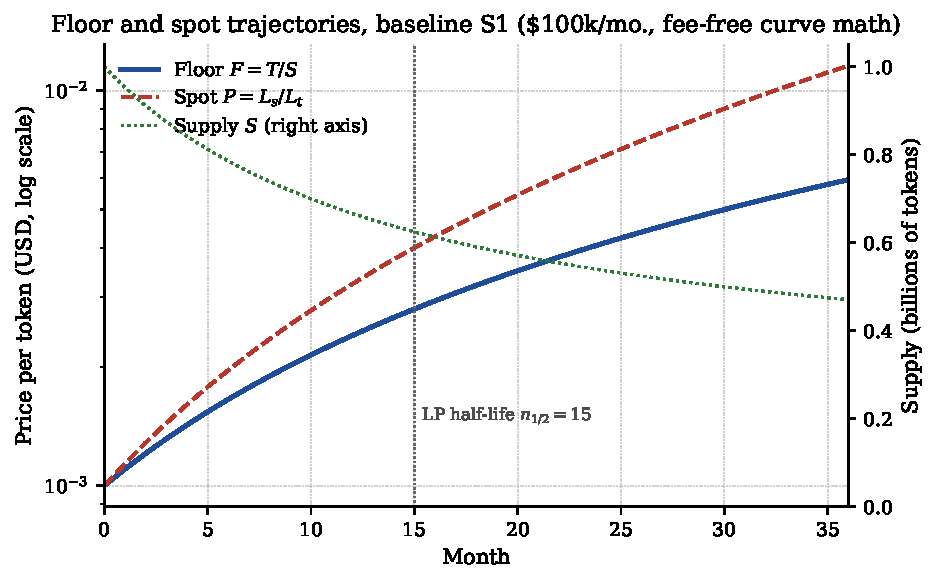
\includegraphics[width=0.55\textwidth]{fig-floor-trajectory.pdf}
\caption{Floor (solid blue), spot (dashed red), and supply (right axis, dotted green) under baseline S1 over a 36-month horizon. The vertical guide at month 15 marks the LP half-life predicted by Theorem~\ref{thm:lp-half-life}; spot diverges from floor monotonically, reaching $\Spot/\Floor \approx 1.94$ at month 36.}
\label{fig:floor-trajectory}
\end{figure}

\paragraph{Adversarial scenarios and design-space sweep.} \emph{S2 (revenue stops)}: $R \to 0$ at $t_{\text{stop}} \in \{6, 12, 24\}$; floor constant onward (Theorem~\ref{thm:spot-floor-convergence}~(1)); redemption channel unaffected. \emph{S3 (mass redemption)}: $\{25\%, 50\%, 75\%\}$ of supply at month 12; funding ratio $= 1.0$ to within the integer residual (Lemma~\ref{lem:integer-redemption}). \emph{S4 (mass dump)}: spot collapses, $\Phit$ fills, the next \texttt{collectFees} steps the floor by the closed-form of Section~\ref{sec:formal-invariants}. \emph{S5 (adversarial-mixed)}: the saturated mixed strategy of Theorem~\ref{thm:bank-run}~(2); yield surface and saturation locus $\alpha = A^*/N$ in Figure~\ref{fig:attacker-phasediagram}. \emph{S6 (organic-volume)}: $V \in \{\$10\text{k}, \$50\text{k}, \$200\text{k}, \$500\text{k}, \$1\text{M}\}$/month; fee-source parity with each revenue-funded leg at $V \approx \$2.3$M/month. Revenue, LP-split, fee-asymmetry, and Monte Carlo sweep figures are in the Zenodo artifact.

\begin{figure}[t]
\centering
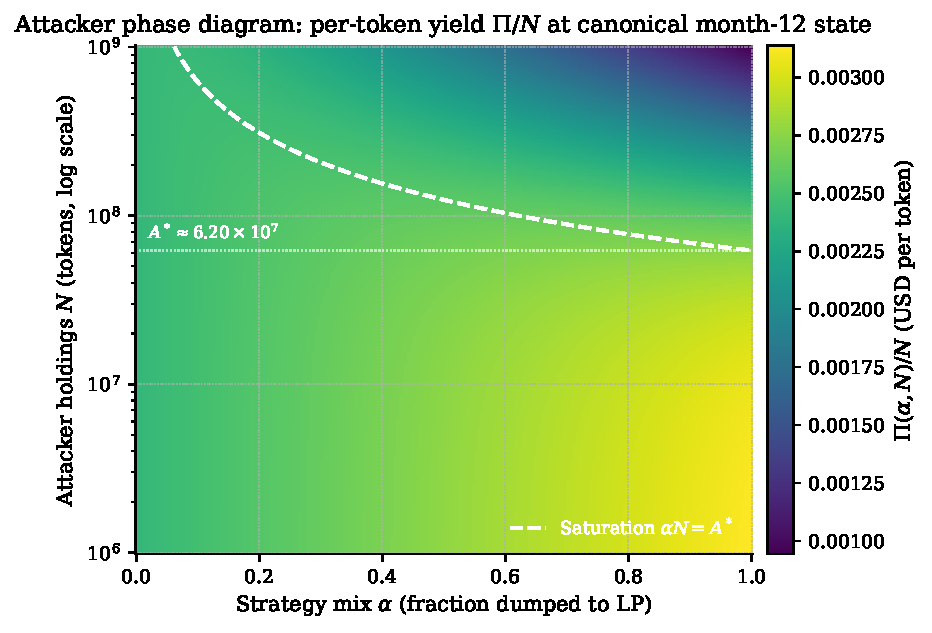
\includegraphics[width=0.55\textwidth]{fig-attacker-phasediagram.pdf}
\caption{Attacker phase diagram at the canonical month-12 state. Heatmap of $\Pi(\alpha, N)/N$ on an $(\alpha, N)$ grid with $N$ on log scale from $10^6$ to $10^9$ tokens. The white dashed curve is the saturation locus $\alpha = A^*/N$ from Theorem~\ref{thm:bank-run} with $A^* \approx 6.20 \cdot 10^7$. Below $N = A^*$ the optimum is $\alpha = 1$ (pure dump); above, the optimum lies on the saturation curve.}
\label{fig:attacker-phasediagram}
\end{figure}

\paragraph{Cross-protocol comparison.} Table~\ref{tab:protocol-comparison} positions M\textsuperscript{2} against five DeFi comparators---OHM \citep{OlympusDAO2021}, RAI \citep{Reflexer2021}, Frax \citep{Frax2021}, Liquity \citep{Liquity2021}, Dai \citep{Maker2019}---and the canonical TradFi closed-end-fund row.

\begin{table}[t]
\centering
\scriptsize
\caption{Comparison matrix across seven design dimensions. ``Fixed supply'' refers to whether the protocol can mint new units of the primary asset post-genesis. ``On-chain redemption'' is a contractually enforceable exit at a protocol-defined price (versus secondary-market only). ``Floor invariant'' indicates whether a per-unit reserve claim is non-decreasing by contract. ``Op. dep.'' indicates whether the protocol's growth (not its safety) depends on a centralized off-chain actor.}
\label{tab:protocol-comparison}
\renewcommand{\arraystretch}{1.18}
\begin{tabular}{p{1.5cm} p{1.25cm} p{1.55cm} p{1.4cm} p{1.5cm} p{1.4cm} p{1.0cm} p{1.85cm}}
\toprule
\textbf{Protocol} & \textbf{Fixed supply?} & \textbf{On-chain redemption?} & \textbf{Treasury composition} & \textbf{Floor invariant?} & \textbf{Gov.} & \textbf{Op. dep.} & \textbf{Primary risk} \\
\midrule
M\textsuperscript{2} & Yes; supply only decreases & Yes; at $\Floor = \Tres/\Sup$ & Single exog.\ stable; one-way in & Yes; non-decreasing by Thm~\ref{thm:floor-monotonicity} & None & Growth only & Smart-contract bug; stable issuer \\
OHM (OlympusDAO) & No; staking rebases up & No (governance vote-gated burn proposals only) & Multi-asset; rebalance by governance & No (``RFV per token'' is rhetorical) & Active gov. & Low (community treasury) & Confidence collapse; gov.\ capture \\
RAI (Reflexer) & No; PID mint/burn & Yes; against ETH at redemption price & ETH collateral via Safe vaults & No (redemption price mean-reverts) & Minimal & None & Oracle manip.; vault liquidation cascade \\
Frax & No; algorithmic + collateralized & Yes; against AMO-managed reserves & Multi-stable + algorithmic & No (peg target, not floor) & Active gov. & Mod. & Peg loss; AMO mispricing \\
Liquity (LUSD) & No; mintable against ETH & Yes; against ETH at \$1 + 0.5\% fee & ETH-only via troves & No (peg target, not floor) & None & None & ETH price crash + recovery-mode cascade \\
MakerDAO (Dai) & No; CDP-style mint & Yes; CDP unwind only & Multi-collateral & Limited (per-vault) & Active gov. & Low & Black-swan oracle deviation; gov.\ capture \\
\midrule
TradFi CEF (closed-end fund) & Effectively yes & No (secondary market only) & Multi-asset, manager-discretion & No (NAV fluctuates; persistent discount) & Board / sh. & Yes (manager) & Discount-to-NAV persistence; mgmt.\ extraction \\
\bottomrule
\end{tabular}
\end{table}

\emph{What the table shows.} Three dimensions discriminate M\textsuperscript{2}: (i) \emph{floor invariance}---only M\textsuperscript{2} contractually enforces a non-decreasing per-unit reserve claim (OHM's ``RFV'' is rhetorical, RAI mean-reverts, Frax/Liquity target pegs, Dai has only per-vault floors, CEFs publish NAV without redemption); (ii) \emph{supply discipline}---only M\textsuperscript{2} guarantees post-genesis supply can only decrease; (iii) \emph{governance surface}---M\textsuperscript{2} and Liquity are the only governance-free entries, but M\textsuperscript{2}'s asset is not a stablecoin and its reserve is external. The CEF row anchors the cross-domain comparison: the persistent discount-to-NAV \citep{LeeShleiferThaler1991,Pontiff1996} arises from the absence of contractual NAV-redemption; M\textsuperscript{2} adds NAV monotonicity, which has no TradFi analog.

\paragraph{Reproducibility.} MIT-licensed simulator at Zenodo DOI \href{https://doi.org/10.5281/zenodo.20255141}{\texttt{10.5281/zenodo.20255141}}, tag \texttt{v0.2.0-paper-v2}: \texttt{make reproduce} regenerates every figure/table from pinned seeds; \texttt{make verify} runs Track A, Track B, the agreement gate, and writes a SHA-256 manifest.

% ============================================================
\section{Limitations and Open Problems}
\label{sec:limitations}

\paragraph{Residual risks.} The protocol is immutable: no upgrade path, admin pause, or governance hook can deploy a bug fix; standard mitigation (external review, integer-reference differential testing, the (P1) Halmos/Certora path) bounds but does not eliminate contract risk. Issuer-side freeze (the March 2023 USDC depeg is canonical) is undefendable; mitigation is restricted to the deployer's choice of stable. Floor \emph{growth} depends on continued revenue: under cessation, Theorem~\ref{thm:spot-floor-convergence} shows graceful CEF-analog degradation, but operator fraud (revenue collected but routed elsewhere) is outside the on-chain threat model and addressed by entity-level disclosure. LP exhaustion under sustained buy-and-burn (Theorem~\ref{thm:lp-half-life}) is intentional: any refill requires either post-genesis minting (violating supply-only-decreases) or treasury redeposit, which lowers the floor since $(\Tres - X)/(\Sup + Y) < \Tres/\Sup$. Regulatory classification is jurisdiction-specific and out of scope.

\paragraph{(P1) End-to-end mechanized verification.} Theorem~\ref{thm:floor-monotonicity} is on paper; discharging it on the deployed bytecode under Halmos or Certora \citep{Tolmach2022} is follow-up work.

\paragraph{(P2) Quantitative LVR/floor-capture identity.} Promoting Conjecture~\ref{conj:lvr-capture} to a theorem requires reconciling LVR's per-unit-time stochastic formulation with M\textsuperscript{2}'s discrete-event floor framing and per-leg fee accounting.

\paragraph{(P3) Sequenced bank-run strategies.} Characterizing the supremum across the full sequenced-strategy class (interleaved LP dumps, \texttt{collectFees}, redemptions within/across blocks) requires modeling the \texttt{collectFees}-bounty equilibrium and v4 fee-realization dynamics.

% ============================================================
\section{Conclusion}
\label{sec:conclusion}

M\textsuperscript{2} enforces a contractually monotone non-decreasing redemption floor over an immutable four-contract operation set: fully specified (C1), proved against the complete operation set with integer-arithmetic residual (C2; Theorem~\ref{thm:floor-monotonicity}, Lemma~\ref{lem:integer-redemption}, Theorems~\ref{thm:redemption-fairness}, \ref{thm:bank-run}), and quantitatively characterized by a two-track simulator with paper-stopping agreement (C3). Three follow-ups: a post-deployment empirical event study; mechanized verification under Halmos/Certora (P1); and immutability-respecting variants (multi-stable backing, operator bonding, dynamic fees).


% ============================================================
\section*{Acknowledgments}
The author thanks Hamed Kalantari Sarcheshmeh and Sina Hashemi for informal review and feedback on early drafts of this work. Any remaining errors are the author's own.

\section*{Disclosures}

\paragraph{Funding.} This research was conducted independently by the author without external funding.

\paragraph{Conflict of interest.} The author intends to deploy a reference implementation of the M\textsuperscript{2} protocol described in this paper. The mechanism is intended for open-source release as a non-proprietary tokenomics primitive available to any DeFi project; the author claims no proprietary rights over the design and does not hold a financial interest in any specific instance of the protocol beyond the reference deployment. Readers should weigh this intended deployment when interpreting the qualitative framing of the paper, though all quantitative claims are derivable from the protocol specification and the closed-form analysis of Sections~\ref{sec:formal-invariants} and~\ref{sec:economic-analysis} and do not depend on any operational assumption about a specific deployment.

\paragraph{Code and data availability.} Simulator, figure scripts, and reference contracts will be released open-source at the Zenodo DOI in the abstract under git tag \texttt{v0.2.0-paper-v2}.

% ============================================================
{\footnotesize
\bibliographystyle{plainnat}
\bibliography{references}
}

\appendix

% ============================================================
\section{Symbol Table}
\label{app:symbols}

Subscripts $(\cdot)_0$ denote genesis values; superscript $(\cdot)^*$ denotes an equilibrium or optimum.

\begin{table}[t]
\centering
\scriptsize
\setlength{\tabcolsep}{4pt}
\renewcommand{\arraystretch}{0.92}
\caption{Notation used throughout the paper.}
\label{tab:symbols}
\begin{tabular}{p{2.4cm} p{12.0cm}}
\toprule
\textbf{Symbol} & \textbf{Meaning} \\
\midrule
$\Tres$ & Treasury stablecoin balance (stable's smallest unit) \\
$\Sup$ & Total token supply (LP + vesting + circulating), in $10^{-18}$-token units \\
$\Lt, \Ls$ & Active LP reserves (token, stable) on the protocol-owned v4 position \\
$\Floor = \Tres/\Sup$ & Floor (redemption) price; 18-decimal fixed-point regardless of stable's decimals \\
$\Spot = \Ls/\Lt$ & AMM spot price \\
$\kInv = \Lt \Ls$ & Constant-product invariant \\
$\Phit, \Phis$ & Raw unrealized fee mass on LP (token, stable), awaiting next \texttt{collectFees} \\
$\Kreal, \Ureal$ & Realized fee mass at \texttt{collectFees}; $(\Kreal, \Ureal) = (\Phit, \Phis)$ at realization \\
$K_{\text{burn}}, U_{\text{treas}}$ & Net burn / net treasury inflow after $0.25\%$ caller bounty \\
$K_b, U_b$ & Caller bounty (token, stable) \\
$f_b, f_s$ & Hook fees on buys ($0.10\%$) and sells ($3\%$) \\
$N$ & Token quantity (attacker or holder) \\
$N_{\text{in}}, X_{\text{in}}$ & Token input to sell swap; stable input to buy swap \\
$B$ & Monthly buy-and-burn size ($B = R/2$ at $50/50$ split) \\
$R$ & Monthly revenue via \texttt{routeRevenue} \\
$A^*, \Delta^*$ & Saturation quantity and run premium (Theorem~\ref{thm:bank-run}); state-only constants \\
$n_{1/2}$ & LP token-side half-life (Theorem~\ref{thm:lp-half-life}); $n_{1/2} = L_{s,0}/B$ \\
$\Delta t^*, \beta, g$ & Inter-call interval, fee-accumulation rate, gas+search cost (Theorem~\ref{thm:collect-equilibrium}) \\
$\Qprec = 10^{18}$, $\dstab, \Qstab = 10^{\dstab}$ & 18-decimal scale; stable's decimals and smallest-unit scale \\
$\contractEval{\cdot}$ & Contract-faithful integer evaluation (vs.\ abstract rational) \\
$\mathrm{Ops}$ & Protocol operation set (Section~\ref{sec:formal-invariants}, Eq.~\eqref{eq:ops}) \\
\bottomrule
\end{tabular}
\end{table}

% ============================================================
\section{Auxiliary Theorems}
\label{app:auxiliary}

MEV-leakage upper bound on protocol buy-and-burn (Section~\ref{sec:protocol}).

\begin{theorem}[MEV Leakage Upper Bound]
\label{thm:mev-bound}
Let $p \in [0, 1]$ be the probability that a buy-and-burn transaction is included via a private (sealed) route, $N_{\text{TWAP}}$ the TWAP granularity, and $B$ the monthly buy size in stable. Let $\varepsilon_{\text{pub}}(M, \Ls)$ denote the public-mempool sandwich efficiency for a swap of size $M$ against stable reserves $\Ls$, satisfying $\varepsilon_{\text{pub}}(M, \Ls) = O(M/\Ls)$ in the small-impact regime. Then the expected MEV leakage on the monthly buy satisfies
\begin{equation}
\mathbb{E}[\mathrm{MEV}] \;\leq\; (1 - p) \cdot \varepsilon_{\text{pub}}(B/N_{\text{TWAP}}, \Ls) \cdot B \;+\; p \cdot \varepsilon_{\text{priv}} \cdot B,
\label{eq:mev-bound}
\end{equation}
where $\varepsilon_{\text{priv}}$ is the (small) private-mempool sandwich efficiency under builder-collusion risk. In particular, for fixed $p$, $\mathbb{E}[\mathrm{MEV}]/B \to p \varepsilon_{\text{priv}}$ as $N_{\text{TWAP}} \to \infty$.
\end{theorem}

\begin{proof}[Proof sketch]
With probability $p$ the transaction is in the private channel where only builder-collusion-level adversaries can sandwich, with efficiency $\varepsilon_{\text{priv}}$; with probability $1 - p$ it is in the public mempool where the searcher can sandwich the swap, with efficiency $\varepsilon_{\text{pub}}$ in the swap's quadratic-impact order. Splitting the monthly buy into $N_{\text{TWAP}}$ equal parts reduces each sub-buy's impact to $B/N_{\text{TWAP}}$, on which the sandwich extracts $\varepsilon_{\text{pub}}(B/N_{\text{TWAP}}, \Ls) \cdot B/N_{\text{TWAP}}$, aggregated over $N_{\text{TWAP}}$ sub-buys; the linearity of expectation gives the first term in~\eqref{eq:mev-bound}. The private leg contributes the second term. $\qed$
\end{proof}

At canonical parameters ($B = \$50\text{k}/\text{month}$, $\Ls \in [\$0.75\text{M}, \$2\text{M}]$, $p \approx 0.95$ on Ethereum mainnet via Flashbots Protect, $N_{\text{TWAP}} = 8$), \eqref{eq:mev-bound} predicts $\mathbb{E}[\mathrm{MEV}]/B \lesssim 0.5\%$, well under a $1\%$-of-revenue target. Multi-block MEV under builder collusion is out of scope (Sections~\ref{sec:protocol},~\ref{sec:limitations}).

\end{document}
